\section{Tiered Compilation in Hotspot}
\label{sec:tiered}
As mentioned in the introduction, Programming Language Virtual Machines like Java Hotspot feature a multi-tier system when compiling methods during execution. 
Java VM's typically use Java Bytecode as input, a platform independent intermediate code generated by a Java Compiler like \texttt{javac}.
The Bytecode is meant to be interpreted by the virtual machine or further compiled into platform dependend machine code.
Hotspot includes one interpreter and two different compilers with different profiling levels resulting in a total of 5 different levels. The following Figure \ref{fig:hs_tiers} gives a short overview as well as showing the standard transitions.
\begin{figure}[h]
  \begin{center}
    \centering
    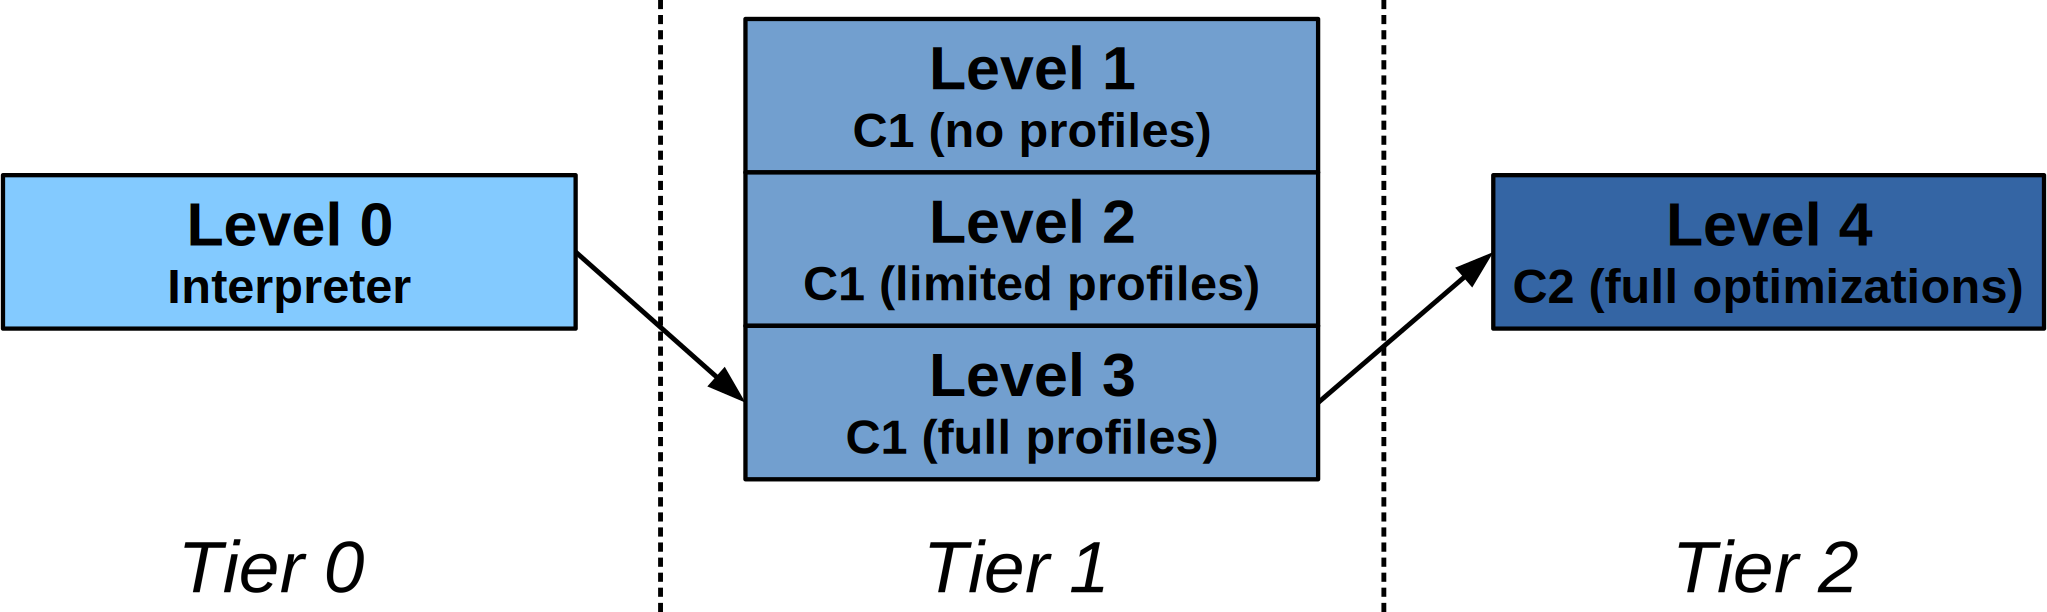
\includegraphics{figures/hs_tiers.png}
    \caption{Overview over compilation tiers}
    \label{fig:hs_tiers}
  \end{center}
\end{figure}

All methods start being executed by Tier-0 also called the Interpreter.
The interpreter is template-based meaning for each bytecode instruction it emits a predefined assembly code snippet.
During execution this code is also profiled. This means method execution counters, loop back-branches and additional statistics are counted. More importantly information about the program flow and state are gathered. These information contain for example which branches get taken or the final types of dynamically typed objects. Once one these counters exceed a predefined, constant threshold the method is considered \textit{hot} which usually results in a compilation at a higher tier.
\\\\
The standard behavior of Hotspot is to proceed with Level 3 (Tier 1). This means the method gets compiled with C1, also referred to as \textit{client} compiler, and continues gathering full profiles.
C1's goal is to provide a fast compilation with a low memory footprint.
The client compiler performs simple optimizations such as constant folding, null check elimination and method inlining.
More information about C1 can be found in \cite{client_compiler_talk} and \cite{client_compiler}.
The levels 1 and 2 include the same optimization but offer no or less profiling information and are used in special cases, for example if the compiler is already very busy or enough profiles are already available.
\\\\
Eventually, when further compile thresholds are exceeded, the JVM further compiles the method with C2, also known as \textit{server} compiler.
The server compiler makes use of the gathered profiles in Tier 0 and Tier 1 and produces highly optimized code. C2 includes far more optimizations like loop unrolling, common subexpression elimination and elimination of range and null checks. It performs optimistic method inlining, for example by converting some virtual calls to static calls.
A more detailed look at the server compiler can be found in \cite{server_compiler}.
\\\\
The naming scheme \textit{client/server} comes from back in the days were tiered compilation was not available and one had to choose the compiler via a Hotspot command line flag. The \textit{Client} compiler was meant to be used for interactive client programs with graphical user interfaces where response time is more important than peak performance. For long running server applications, the highly optimized but slower server compiler was used. 
\\\\
Tiered compilation was introduced to improve start-up performance of the JVM.
Starting with the interpreter means that there is zero wait time until the method is executed since one does not need to wait until a compilation is finished. C1 allows the JVM to have more optimized of the code available early which then can be used to create a richer profile to be used when compiling with C2. Ideally this profile already contains most of the program flow so less deoptimizations (see \ref{sec:deoptimizations} occur.

\section{On Stack Replacement}
\label{sec:onstackreplacement}
Since the JVM does not only count method invocations but also loop back branches (see also Section \ref{sec:compilethresholds}) it can happen that a method gets compiled while it is still running and the compiled method is ready before the method has finished.
Instead of waiting for the next method invocation Hotspot can replace the method directly on the stack (see Figure \ref{fig:osr}) and is called \textit{on stack replacement}.
An example would be a simple method consisting of a very long running loop.
\begin{figure}[h]
  \begin{center}
    \centering
    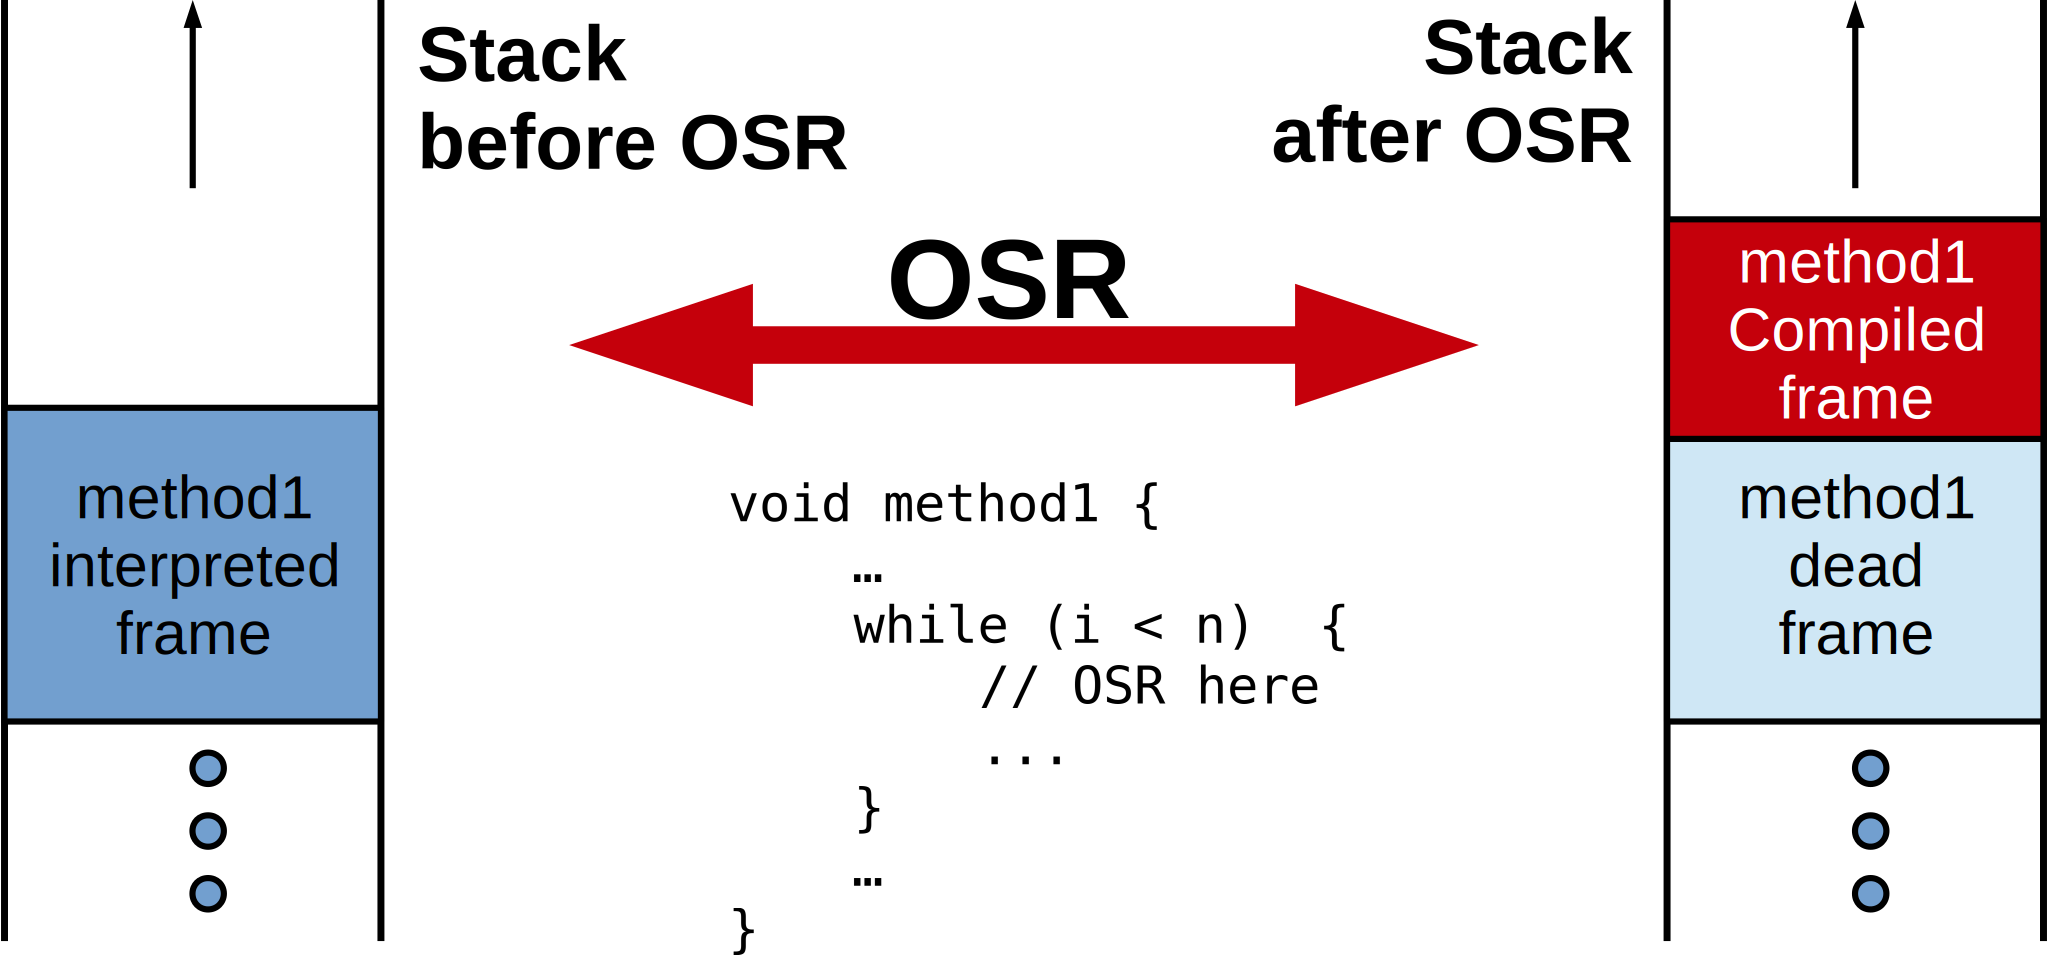
\includegraphics{figures/osr.png}
    \caption{Overview over compilation tiers}
    \label{fig:osr}
  \end{center}
\end{figure}

\section{Deoptimizations}
\label{sec:deoptimizations}
Ideally we compile a method with as much profiling information as possible.
Since the profiling information are usually gathered in levels 0 and 3 it can happen that a method compiled by C2 wants to execute a branch it never used before.
In this case the information about this branch are not available in the profile and therefore have not been compiled into the C2-compiled code.
This is done to allow further, very optimistic optimization and to keep the compiled code smaller. So instead, the compiler places an uncommon trap at unused branches or unloaded classes which will get triggered in case they actually get used at a later time in execution.
\\\\
The JVM then stops execution of that method and returns the control back to the interpreter. This process is called \textit{deoptimization} and considered very costly. The previous interpreter state has to be restored and eventually the method might get recompiled with the newly gained information.

\section{Compile Thresholds}
\label{sec:compilethresholds}
The transitions between the compilation levels (see Fig. \ref{fig:hs_tiers}) are chosen based on predefined constants called \textit{compile thresholds}. When running an instance of the JVM one can specify them manually or use the ones provided. A list of thresholds and their default values relevant to this thesis are given in Appendix \ref{app:compilethresholds}.
The standard transitions from Level 0 to 3 and 3 to 4 happen when the following predicate returns true:
\begin{align*}
& i > TierXInvocationThreshold \ * \ s \\
 || \ (&i > TierXMinInvocationThreshold \ * \ s \ \&\& \ i \ + \ b \ > \ TierXCompileThreshold \ * \ s) 
\end{align*}
where $X$ is the next compile level (3 or 4), $i$ the number of method invocations, $b$ the number of backedges and $s$ a scaling coefficient (default = 1).
The thresholds are relative and individual for interpreter and compiler.
\\\\
On Stack Replacement uses a simpler predicate:
$$b > TierXBackEdgeThreshold * s$$

Please note that there are further conditions influencing the compilation like the load on the compiler which will not be discussed further.

\section{Examples}

I will continue with presenting three very simple examples that illustrate the usage and benefit from using cached profiles. To start I will consider a standard Java Hotspot execution with OnStackReplacement disabled.
\\\\
Example one is a simple class that invokes a method one hundred times. The method itself consists of a long running loop. The source code is shown in Listing \ref{l:nocompile}.
Since OSR is disabled and a compilation to level 3 is triggered after 200 invocations this method will never leave the interpreter. 
\lstset{numbers=left, numberstyle=\tiny, stepnumber=1, numbersep=5pt}
\lstset{basicstyle=\ttfamily}
\lstset{frame=tb}
\begin{lstlisting}[float,caption=Example usage of the listing package,label=l:nocompile,language=Java]
class NoCompile {
    double result = 0.0;
    for(int c = 0; c < 100; c++) {
      result = method1(result);
    }
    public double method1(double count) {
        for(int k = 0; k < 10000000; k++) {
            count = count + 50000;
        }
   }
}
\end{lstlisting}
